\section{Interface Iteration}\label{interface-iteration}

\begin{figure}[htbp]
\centering
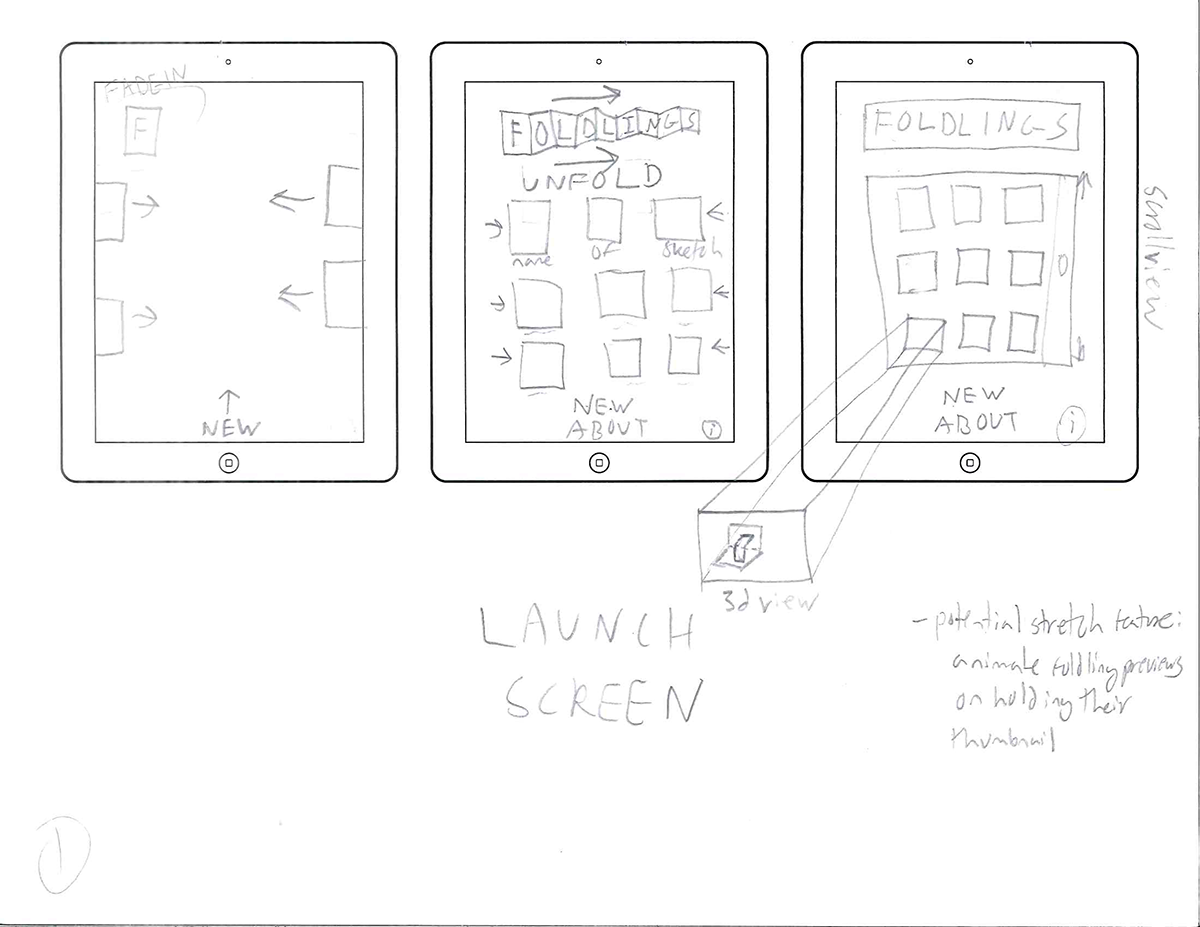
\includegraphics{figures/90_Appendix_UI_Mockups/001.png}
\caption{Initial mockups showing cards for saved sketches on the main
screen.}
\end{figure}

In December 2014, we had a functional prototype of our popup card design
software. Users could create cuts and folds and. However, in many ways
our software was no better than manually creating popup cards. In order
to create a valid and beautiful design, users needed some prior
knowledge. Although we provided. Performance problems also hampered
users' ability to create designs. Our goal was to improve both of these
aspects of Foldlings dramatically, to arrive at an intuitive and
functional tool.

In arriving at our final design, we iterated through several potential
designs, each time getting feedback through informal user studies. We
made many changes to the toolset and experience based on feedback from
users. The final approach is ``feature-based'': in other words, the user
creates multiple cuts and folds in a single action, rather than
individually. These discrete logical units allow the user to design more
quickly, and to combine multiple different feature types to create
complex designs. A key advantage to this design over a less structured
approach is modularity. This is both an algorithmic and an interface
advantage: our algorithms benefit from collecting cuts and folds into
discrete logical units, and the user benefits from a faster and more
structured design process.

\begin{figure}[htbp]
\centering
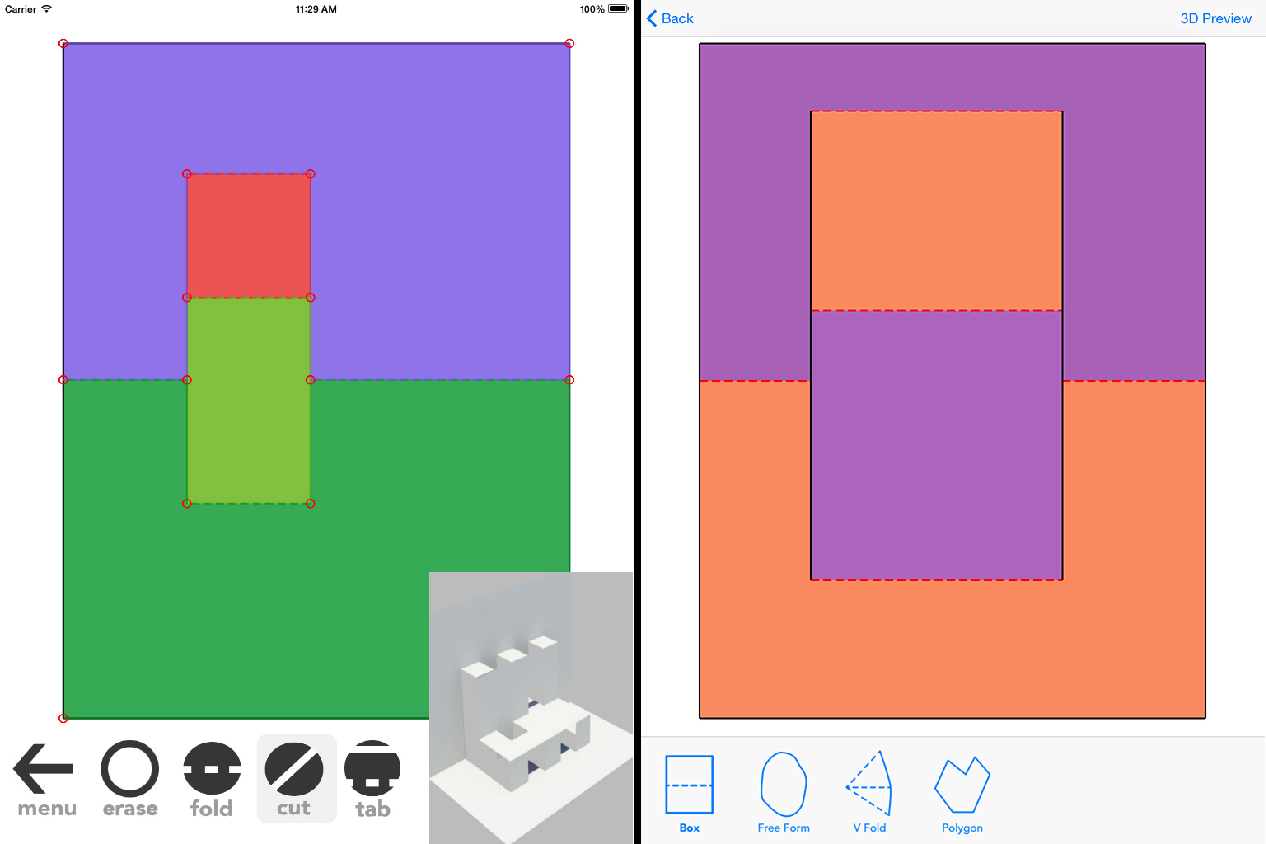
\includegraphics{figures/31_UI_Interface_Iteration/beforeafterinface.pdf}
\caption{Left: drawing interface as of December 2014. Right: drawing
interface as of August 2015.}
\end{figure}

Throughout the development process, we collected feedback through
informal user tests. One test we performed was to present a
partially-implemented version of our software to users. The majority of
buttons were functional --- erase, cut, fold, and and tab, but a few.
The primary goals were to test whether our existing tools were useful
and to collect feedback on potential new features for Foldlings. When a
user tapped a button that we had not yet implemented, we asked them to
describe how they thought the tool would work, and talked with them
about the behavior the button represented. While users created sketches
using our software, we took notes on their experience and collected
their suggestions for improvementss.

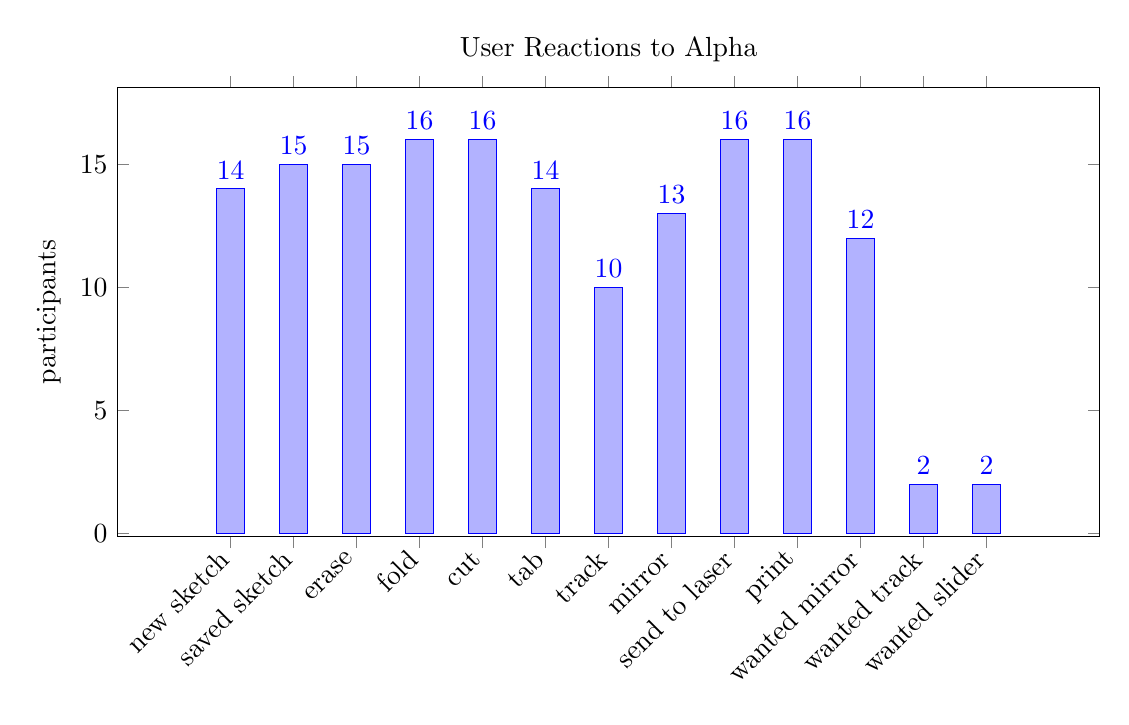
\begin{tikzpicture}
  \begin{axis}[
    title=User Reactions to Alpha,
    ybar,
    enlargelimits=0.15,
    x=0.8cm,
    legend style={at={(0.5,-0.2)},
      anchor=north,legend columns=-1},
    ylabel={participants},
    symbolic x coords={new sketch,saved sketch,erase,fold,cut,tab,track,mirror,send to laser,print,wanted mirror,wanted track,wanted slider},
    xtick=data,
    nodes near coords, 
    nodes near coords align={vertical},
    x tick label style={rotate=45,anchor=east},
    ]
    \addplot coordinates {(new sketch,14)(saved sketch,15)(erase,15)(fold,16)(cut,16)(tab,14)(track,10)(mirror,13)(send to laser,16)(print,16)(wanted mirror,12)(wanted track,2)(wanted slider,2)};
  \end{axis}
\end{tikzpicture}

In the graph above, the first 10 labels indicate the number of
participants who tapped a button. The last three labels --- starting
with ``wanted mirror'' --- show responses to unimplemented tools. To
calculate these numbers, we asked first users to describe what they
thought the button would do, and then . The tally represents a
qualitative measure of whether the user was enthusiastic about the
feature or had a more negative response. Some negative responses include
confusion about the tool's purpose and

From this test, we learned that the track and slider tools were
confusing, and that novice users were generally not interested in
creating features that require multiple pieces of paper.

\textbf{\textgreater{}\textgreater{}TODO: separate user comments from
observation}

\begin{longtable}[c]{@{}l@{}}
\caption{Feedback from first user test.}\tabularnewline
\toprule
\begin{minipage}[b]{0.82\columnwidth}\raggedright\strut
Comments
\strut\end{minipage}\tabularnewline
\midrule
\endfirsthead
\toprule
\begin{minipage}[b]{0.82\columnwidth}\raggedright\strut
Comments
\strut\end{minipage}\tabularnewline
\midrule
\endhead
\begin{minipage}[t]{0.82\columnwidth}\raggedright\strut
want option to fold other way, wanted to be able to draw over existing
line with tab tool, made a cake, crashed on returning to sketch
\strut\end{minipage}\tabularnewline
\begin{minipage}[t]{0.82\columnwidth}\raggedright\strut
track and slider will need explanation; wanted to use non-horizontal
folds
\strut\end{minipage}\tabularnewline
\begin{minipage}[t]{0.82\columnwidth}\raggedright\strut
wanted to fold by pinching, want to rename? delete, move them around?
\strut\end{minipage}\tabularnewline
\begin{minipage}[t]{0.82\columnwidth}\raggedright\strut
wanted ortho views, hold to view info about tool, examples. Interactive
tutorial
\strut\end{minipage}\tabularnewline
\begin{minipage}[t]{0.82\columnwidth}\raggedright\strut
erased master fold, crashing at preview step
\strut\end{minipage}\tabularnewline
\begin{minipage}[t]{0.82\columnwidth}\raggedright\strut
wanted interactive tutorials, made a cat
\strut\end{minipage}\tabularnewline
\begin{minipage}[t]{0.82\columnwidth}\raggedright\strut
momentary confusion getting back to sketch
\strut\end{minipage}\tabularnewline
\begin{minipage}[t]{0.82\columnwidth}\raggedright\strut
wanted to move around existing sketches
\strut\end{minipage}\tabularnewline
\begin{minipage}[t]{0.82\columnwidth}\raggedright\strut
confused about concept of a laser cutter
\strut\end{minipage}\tabularnewline
\begin{minipage}[t]{0.82\columnwidth}\raggedright\strut
wanted interative tutorial
\strut\end{minipage}\tabularnewline
\begin{minipage}[t]{0.82\columnwidth}\raggedright\strut
wanted to fold 3d preview by hand
\strut\end{minipage}\tabularnewline
\begin{minipage}[t]{0.82\columnwidth}\raggedright\strut
very frustrated by tools that aren't implemented yet
\strut\end{minipage}\tabularnewline
\begin{minipage}[t]{0.82\columnwidth}\raggedright\strut
confused by track \& slider
\strut\end{minipage}\tabularnewline
\begin{minipage}[t]{0.82\columnwidth}\raggedright\strut
needed heavy guidance; completely confused by track/slider
\strut\end{minipage}\tabularnewline
\begin{minipage}[t]{0.82\columnwidth}\raggedright\strut
wanted more snapping/guidance on creating valid designs
\strut\end{minipage}\tabularnewline
\begin{minipage}[t]{0.82\columnwidth}\raggedright\strut
fairly self-sufficient after tools were explained, made a house, moved
slowly, waiting for planes to calculate
\strut\end{minipage}\tabularnewline
\bottomrule
\end{longtable}
